\documentclass{beamer}
\usefonttheme{professionalfonts}

\usetheme[secheader]{PaloAlto}
%\usecolortheme{structure}
%\usepackage[latin1]{inputenc}

\title{The Bayesian viewpoint}
\subtitle{An introduction}
\author{Hari A Ravindran}
\date{August 11, 2017}
%\institute[2014]{a.k.a. A Tale of Three Methods}

\makeatletter
  \setbeamertemplate{sidebar \beamer@sidebarside}%{sidebar theme}
  {
    \beamer@tempdim=\beamer@sidebarwidth%
    \advance\beamer@tempdim by -6pt%
    \insertverticalnavigation{\beamer@sidebarwidth}%
    \vfill
    \ifx\beamer@sidebarside\beamer@lefttext%
    \else%
      \usebeamercolor{normal text}%
      \llap{\usebeamertemplate***{navigation symbols}\hskip0.1cm}%
      \vskip2pt%
    \fi%
}%

\makeatother

\usepackage{amsmath,amsfonts,amsthm,amssymb,amscd}
\usepackage{mathtools}
\usepackage{relsize}
\usepackage{enumerate}
\usepackage{empheq}
\usepackage{mathrsfs}
\usepackage{latexsym}
\input amssym.def
\input amssym.tex


    %=======================================================
    %   THIS IS WHERE YOU PUT SHORTCUT DEFINITIONS
    %========================================================

% Note that we use a percent sign to comment out a line
% below are shortcut commands

%%%%%%%%%%%%%%%%%%%%%%%%%%%%%%%%%%%%%%%%%%%%%%%
% below are shortcuts for equation, eqnarray,
% itemize and enumerate environments

\newcommand\be{\begin{equation}}
\newcommand\ee{\end{equation}}
\newcommand\bea{\begin{eqnarray}}
\newcommand\eea{\end{eqnarray}}
\newcommand\bi{\begin{itemize}}
\newcommand\ei{\end{itemize}}
\newcommand\ben{\begin{enumerate}}
\newcommand\een{\end{enumerate}}

%%%%%%%%%%%%%%%%%%%%%%%%%%%%%%%%%%%%%%%%%%%%%%%%
% Theorem / Lemmas et cetera

\newtheorem{thm}{Theorem}[section]
\newtheorem{conj}[thm]{Conjecture}
\newtheorem{cor}[thm]{Corollary}
\newtheorem{lem}[thm]{Lemma}
\newtheorem{prop}[thm]{Proposition}
\newtheorem{exa}[thm]{Example}
\newtheorem{defi}[thm]{Definition}
\newtheorem{exe}[thm]{Exercise}
\newtheorem{rek}[thm]{Remark}
\newtheorem{que}[thm]{Question}
\newtheorem{prob}[thm]{Problem}
\newtheorem{cla}[thm]{Claim}


%%%%%%%%%%%%%%%%%%%%%%%%%%%%%%%%%%%%%%%%%
% shortcuts to environments
% this allows you to do textboldface: simply type \tbf{what you want in bold}

\newcommand{\tbf}[1]{\textbf{#1}}
\newcommand{\arr}[1]{\overrightarrow{#1}}
\newcommand{\avec}[1]{\langle #1 \rangle}

%%%%%%%%%%%%%%%%%%%%%%%%%%%%%%%%%%%%%%%%%%%%%%%%%%
% shortcut to twocase and threecase definitions

\newcommand{\twocase}[5]{#1 \begin{cases} #2 & \text{#3}\\ #4
&\text{#5} \end{cases}   }
\newcommand{\threecase}[7]{#1 \begin{cases} #2 &
\text{#3}\\ #4 &\text{#5}\\ #6 &\text{#7} \end{cases}   }


%%%%%%%%%%%%%%%%%%%%%%%%%%%%%%%%%%%%%%%%%
%Blackboard Letters

\newcommand{\R}{\ensuremath{\mathbb{R}}}
\newcommand{\C}{\ensuremath{\mathbb{C}}}
\newcommand{\Z}{\ensuremath{\mathbb{Z}}}
\newcommand{\Q}{\mathbb{Q}}
\newcommand{\N}{\mathbb{N}}
\newcommand{\F}{\mathbb{F}}
\newcommand{\W}{\mathbb{W}}
\newcommand{\Qoft}{\mathbb{Q}(t)}  %use in linux


%%%%%%%%%%%%%%%%%%%%%%%%%%%%%%%%%%%%%%%%%
% Finite Fields and Groups

\newcommand{\Fp}{ \F_p }


%%%%%%%%%%%%%%%%%%%%%%%%%%%%%%%%%%%%%%%%%
% Fractions

\newcommand{\foh}{\frac{1}{2}}  %onehalf
\newcommand{\fot}{\frac{1}{3}}
\newcommand{\fof}{\frac{1}{4}}

%%%%%%%%%%%%%%%%%%%%%%%%%%%%%%%%%%%%%%%%%
% Legendre Symbols

\newcommand{\js}[1]{ { \underline{#1} \choose p} }


%%%%%%%%%%%%%%%%%%%%%%%%%%%%%%%%%%%%%%%%%
% matrix shortcuts

\newcommand{\mattwo}[4]
{\left(\begin{array}{cc}
                        #1  & #2   \\
                        #3 &  #4
                          \end{array}\right) }

\newcommand{\matthree}[9]
{\left(\begin{array}{ccc}
                        #1  & #2 & #3  \\
                        #4 &  #5 & #6 \\
                        #7 &  #8 & #9
                          \end{array}\right) }

\newcommand{\dettwo}[4]
{\left|\begin{array}{cc}
                        #1  & #2   \\
                        #3 &  #4
                          \end{array}\right| }

\newcommand{\detthree}[9]
{\left|\begin{array}{ccc}
                        #1  & #2 & #3  \\
                        #4 &  #5 & #6 \\
                        #7 &  #8 & #9
                          \end{array}\right| }


%%%%%%%%%%%%%%%%%%%%%%%%%%%%%%%%%%%%%%%%%
% greek letter and Roman Numeral shortcuts

\newcommand{\ga}{\alpha}                  %gives you a greek alpha
\newcommand{\gb}{\beta}
\newcommand{\gep}{\epsilon}
\newcommand{\res}{\text{Res}}
\newcommand{\RNum}[1]{\uppercase\expandafter{\romannumeral #1\relax}}


%%%%%%%%%%%%%%%%%%%%%%%%%%%%%%%%%%%%%%%%%
% Big-O notation shortcut

\newcommand{\BigO}[1]{\ensuremath{\operatorname{O}\left(#1\right)}}

%%%%%%%%%%%%%%%%%%%%%%%%%%%%%%%%%%%%%%%%%
% general functions
\newcommand{\notdiv}{\nmid}               % gives the not divide symbol

%%%%%%%%%%%%%%%%%%%%%%%%%%%%%%%%%%%%%%%%%%
% inmod definition

\makeatletter
\def\inmod#1{\allowbreak\mkern4mu({\operator@font mod}\,\,#1)}
\makeatother

%%%%%%%%%%%%%%%%%%%%%%%%%%%%%%%%%%%%%%%%%%%%%%%%

\begin{document}

\frame{\titlepage}

\section{Introduction}
%\frame{\tableofcontents}

\subsection{On reasoning}
\frame {
	\frametitle{Deductive reasoning}
	\begin{itemize}
	\item<1-> Generally credited to Aristotle's \textit{Organon}. \\~\\
	\item<2-> If $A$ is true, then $B$ is true. \\~\\
	\item<3-> Its inverse: If $B$ is false, then $A$ is false. \\~\\
	\item<4-> Do we always have the right kind of information to allow this kind of reasoning?
	\end{itemize}
}

\frame {
	\frametitle{Plausible reasoning}
	\begin{itemize}
	\item<1-> Not quite. Sometimes, we need weaker syllogisms. \\~\\
	\item<2-> If $A$ is true, then $B$ is true.
	\item<3-> What if we only know that $B$ is true? \\~\\
	\item<4-> We would like to say: Then, $A$ becomes more plausible. \\~\\
	\item<5-> Similar reasoning: If $A$ is false, then $B$ becomes less plausible.
	\end{itemize}
}

\frame {
	\frametitle{Modes of plausible reasoning}
	\begin{itemize}
	\item<1-> Reasoning from consequence.
	\item<2-> Reasoning from randomness.
	\item<3-> Reasoning from analogy. \\~\\
	\item<4-> In the calculus of plausibility, our \textbf{prior} assessments are all important!
	\end{itemize}
}

\subsection{Bayes' theorem}
\frame {
	\frametitle{Prior, likelihood \& posterior}
	\begin{itemize}
	\item<1-> Observed data $D$.
	\item<2-> Want to know something about a variable $\theta$. \\~\\
	\item<3-> Our interest is then in the quantity:

\[ p(\theta|D) = \frac{p(D|\theta) \, p(\theta)} {p(D)} = \frac{p(D|\theta) \, p(\theta)} {\int\limits_{\theta}p(D| \theta) \, p(\theta)}\]

	\item<4-> $p(\theta|D)$ is the \textit{posterior} distribution of the variable $\theta$ in light of the observed data, $p(\theta)$ is the \textit{prior}, and $p(D|\theta)$ is the \textit{generative model/likelihood} of the dataset.
	\end{itemize}
}

\section{An example}

\subsection{Coin flipping}
\frame {
	\frametitle{Exact binomial probability inference}
	\begin{itemize}
	\item<1-> Outcome of a single flip given by a function of parameter $\theta$: 
	
	\[ p(\gamma| \theta) = \theta^{\gamma} \, (1 - \theta)^{(1 - \gamma)} \] \\~\\

	\item<2-> So, if you have $z$ heads out of $N$ flips: 
	
	\[ p(\{ \gamma_i \} | \theta) = \theta^{z} \, (1 - \theta)^{(N - z)} \] \\~\\
	
	where $z$ is $\displaystyle \sum\limits_i \gamma_i$
	\end{itemize}	
	   }

\frame {
	\frametitle{Specifying the prior}
	\begin{itemize}
	\item<1-> Beta distribution: 
	\begin{align}
		p(\theta| a, b) & = \text{beta} (\theta| a, b) \nonumber \\
						& = \theta^{(a-1)} (1 - \theta)^{(b - 1)} / B(a, b)	\nonumber 		 	
	\end{align} \\~\\
	\item<2-> In terms of the mode $\omega$ and concentration $\kappa$,
	\[ a = \omega (\kappa - 2) + 1 \text{ and } b = (1 - \omega)(\kappa - 2) + 1\]
	where $\kappa > 2$
	\end{itemize}	
	   }
	
\frame {
	\frametitle{The posterior}
	\begin{itemize}
	\item<1-> Posterior is also a beta: 
	\begin{align}
		p(\theta| z, N) & = \frac{p(z, N|\theta) \, p(\theta)} {p(z, N)} \nonumber \\ \nonumber ~\\
						& = \theta^{z} \, (1 - \theta)^{N - z} \,\,\, \frac{\theta^{(a-1)} (1 - \theta)^{(b - 1)}} {B(a, b)} \bigg/ p(z, N)	\nonumber \\ \nonumber ~\\
						& = \text{beta}(\theta | z + a, N - z + b) \nonumber 		 	
	\end{align}
	\item<2-> The posterior is a compromise of prior and likelihood.
	\end{itemize}	
	   }
	   	   	   
\frame {
	\frametitle{Example 1}
	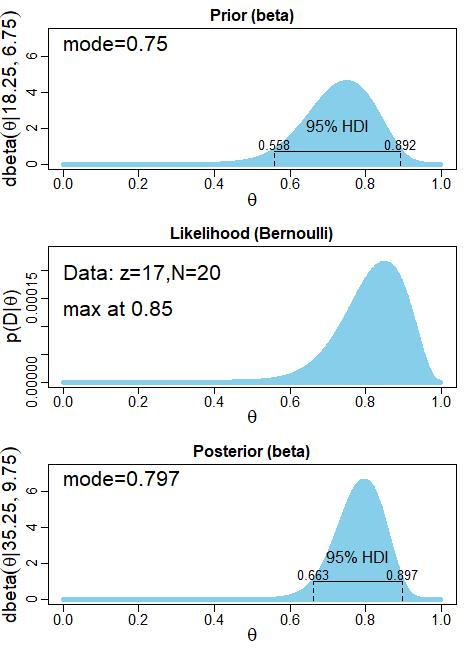
\includegraphics[scale = 0.33]{BernBeta Example1.jpg}	
	   }

\frame {
	\frametitle{Example 2}
	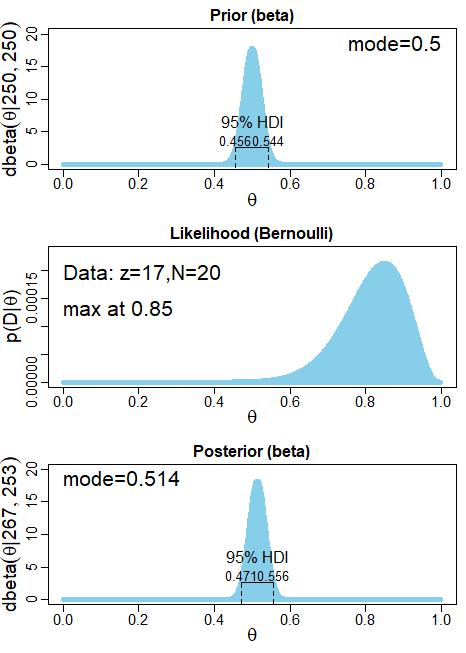
\includegraphics[scale = 0.33]{BernBeta Example2.jpg}	
	   }

\frame {
	\frametitle{Example 3}
	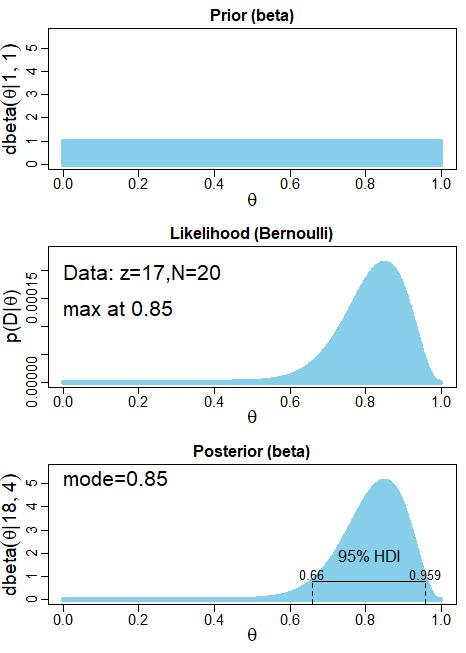
\includegraphics[scale = 0.33]{BernBeta Example3.jpg}	
	   }

\section{Practicalities}

\subsection{Potential issues}
\frame {
	\frametitle{What should we watch out for?}
	\begin{itemize}
	\item<1-> What are your priorities? \\~\\
	\item<2-> Subjective vs. objective priors. \\~\\
	\item<3-> Are analytical solutions always viable? \\~\\
	\item<4-> (Nope!) MCMC methods to the rescue.
	\end{itemize}
	   }
	   	   	   
\subsection{Another example}
\frame {
	\frametitle{Non-beta prior}
	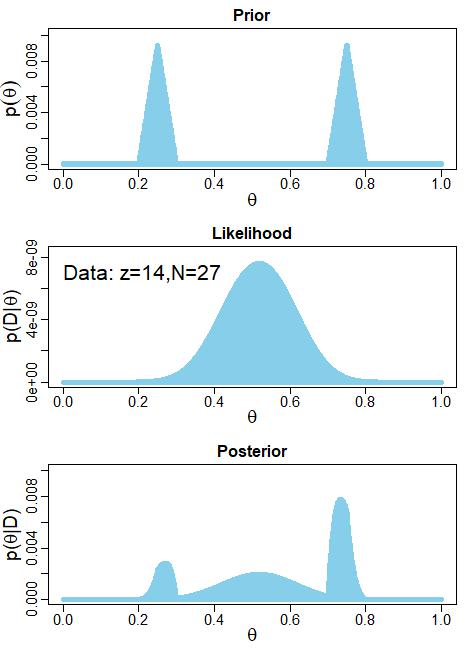
\includegraphics[scale = 0.33]{BernGridExample10.jpg}	
}


\subsection{Conjugate priors}
\frame {
	\frametitle{Conjugate prior distributions}
	\begin{itemize}
	\item<1-> Let $f_{\mu} (x) = e^{n[\alpha \, \bar{x} - \psi(\alpha)]} f_0(x)$, and \\~\\
	\item<2-> $g_{n_0, x_0} (\mu) = c \, e^{n_0[\alpha \, x_0 - \psi(\alpha)]} \bigg/ V(\mu)$.\\~\\
	\item<3-> Then,
	\begin{align}	
	g(\mu|x) &= g_{n_+, \bar{x}_+} (\mu) \text{, where} \nonumber \\
	n_+ &= n_0 + n \text{ and } \bar{x}_+ = \frac{n_0}{n_+} \, x_0 + \frac{n}{n_+} \, \bar{x} \nonumber
	\end{align}
	\end{itemize}	
	   }

\subsection{Empirical Bayes}	   	   
\frame {
	\frametitle{Robbins' Formula}
	 \begin{itemize}
	\item<1-> Consider following claims data for a European automobile insurance company circa 1950s:\\~\\
	\begin{center}
		 \begin{tabular}{||c c c c c c c c c||} 
 		 	\hline
 			Claims & 0 & 1 & 2 & 3 & 4 & 5 & 6 & 7 \\ [0.5ex] 
 			\hline\hline
 			Counts $y_x$ & 7840 & 1317 & 239 & 42 & 14 & 4 & 4 & 1 \\ [1ex] 
 			\hline 
		  \end{tabular}
	\end{center}
	\vspace{25pt}
	\item<2-> \textbf{Key idea} Large data sets of parallel situations carry within them their own Bayesian information.
	\end{itemize}	
	   }
\section{Final thoughts}  
\frame {
	\frametitle{Last but not least}
	\begin{itemize}	
	\item<1-> Bayesian Learning (BIC, etc.) \\~\\
	\item<2-> Frequentist vs. Bayesian comparisons 
	\end{itemize}	
	   }

\end{document}